\begin{name}
	{\tenchude}{ĐỀ ÔN TẬP SỐ 2}{LỚP TOÁN THẦY PHÁT}{\thoigian}
\end{name}
\Opensolutionfile{ans}[ans/ans-Vted-12-2023]

%%==========Câu 1
\begin{ex}%[Đề 12 - Dự án đề VTED 2023 - Đợt 2 - Đoàn Minh Tân]%[2H1Y3-2]
	Một khối chóp có diện tích đáy bằng $12$ và chiều cao bằng $4$. Thể tích của khối chóp đó bằng
	\choice
	{$48$}
	{$144$}
	{\True $16$}
	{$24$}
	\loigiai{
	Thể tích khối chóp đã cho là $V=\dfrac{1}{3}Bh=\dfrac{1}{3}\cdot 12\cdot 4=16$.
	}
\end{ex}
%%==========Câu 2
\begin{ex}%[Đề 12 - Dự án đề VTED 2023 - Đợt 2 - Đoàn Minh Tân]%[2D1Y5-7]
	Điểm nào dưới đây thuộc đồ thị hàm số $y=x^3-x^2+x-1$?
	\choice
	{$P(-2;1)$}
	{$N(-3;-2)$}
	{$M(1;2)$}
	{\True $Q(2;5)$}
	\loigiai{
	Ta có $y(-2)=-15$; $y(-3)=-40$; $y(1)=0$; $y(2)=5$.\\
	Vậy điểm $Q(2;5)$ thuộc đồ thị hàm số đã cho.
	}
\end{ex}
%%==========Câu 3
\begin{ex}%[Đề 12 - Dự án đề VTED 2023 - Đợt 2 - Đoàn Minh Tân]%[2D2Y4-1]
	Hàm số nào sau đây có tập xác định là $\mathbb{R}$?
	\choice
	{$y=x^{-3}$}
	{$y=\log_3 x$}
	{\True $y=\left(\dfrac{3}{2}\right)^x$}
	{$y=x^{\tfrac{3}{2}}$}
	\loigiai{
	Hàm số $y=x^{-3}$ có tập xác định là $\mathscr{D}=\mathbb{R}\setminus \{0\}$.\\
	Hàm số $y=\log_3 x$ có tập xác định là $\mathscr{D}=(0;+\infty)$.\\
	Hàm số $y=\left(\dfrac{3}{2}\right)^x$ có tập xác định là $\mathscr{D}=\mathbb{R}$\\
	Hàm số $y=x^{\tfrac{3}{2}}$ có tập xác định là $\mathscr{D}=(0;+\infty)$.
	}
\end{ex}
%%==========Câu 4
\begin{ex}%[Đề 12 - Dự án đề VTED 2023 - Đợt 2 - Đoàn Minh Tân]%[2D2Y5-1]
	Tập nghiệm của phương trình $\log_2(2x-3)=3$ là
	\choice
	{\True $S=\left\lbrace \dfrac{11}{2}\right\rbrace$}
	{$S=\left\lbrace \dfrac{9}{2}\right\rbrace$}
	{$S=\left\lbrace 6\right\rbrace$}
	{$S=\left\lbrace 3\right\rbrace$}
	\loigiai{
	Ta có $\log_2(2x-3)=3\Leftrightarrow 2x-3=2^3\Leftrightarrow 2x-3=8\Leftrightarrow x=\dfrac{11}{2}$.\\
	Vậy phương trình có tập nghiệm $S=\left\lbrace \dfrac{11}{2}\right\rbrace$.
	}
\end{ex}
%%==========Câu 5
\begin{ex}%[Đề 12 - Dự án đề VTED 2023 - Đợt 2 - Đoàn Minh Tân]%[2H2Y1-2]
	Diện tích xung quanh $S_{\text{xq}}$ của hình trụ có bán kính đáy $r$ và độ dài đường sinh $\ell$ là
	\choice
	{$S_{\text{xq}}=\pi r\ell$}
	{$S_{\text{xq}}=\dfrac{1}{3}\pi r\ell$}
	{\True $S_{\text{xq}}=2\pi r\ell$}
	{$S_{\text{xq}}=\dfrac{1}{2}\pi r\ell$}
	\loigiai{
	Diện tích xung quanh $S_{\text{xq}}$ của hình trụ đã cho là $S_{\text{xq}}=2\pi r\ell$.
	}
\end{ex}
%%==========Câu 6
\begin{ex}%[Đề 12 - Dự án đề VTED 2023 - Đợt 2 - Đoàn Minh Tân]%[2D4Y1-1]
	Mô-đun của số phức $z=4-3i$ bằng
	\choice
	{$7$}
	{$\sqrt{7}$}
	{$25$}
	{\True $5$}
	\loigiai{
	Ta có $z=4-3i\Rightarrow |z|=\sqrt{4^2+(-3)^2}=5$.
	}
\end{ex}
%%==========Câu 7
\begin{ex}%[Đề 12 - Dự án đề VTED 2023 - Đợt 2 - Đoàn Minh Tân]%[2H3Y3-2]
	Trong không gian $Oxyz$, phương trình của đường thẳng đi qua điểm $M(-1;0;2)$, đồng thời nhận véc-tơ $\overrightarrow{u}=(2;3;-1)$ làm véc-tơ chỉ phương là
	\choice
	{\True $\dfrac{x+1}{2}=\dfrac{y}{3}=\dfrac{z-2}{-1}$}
	{$\dfrac{x-1}{2}=\dfrac{y}{3}=\dfrac{z+2}{-1}$}
	{$\dfrac{x-1}{2}=\dfrac{y}{3}=\dfrac{z+2}{1}$}
	{$\dfrac{x+1}{2}=\dfrac{y}{3}=\dfrac{z-2}{1}$}
	\loigiai{
	Đường thẳng đi qua điểm $M(-1;0;2)$ và có véc-tơ chỉ phương $\overrightarrow{u}=(2;3;-1)$ có phương trình $\dfrac{x+1}{2}=\dfrac{y}{3}=\dfrac{z-2}{-1}$.
	}
\end{ex}
%%==========Câu 8
\begin{ex}%[Đề 12 - Dự án đề VTED 2023 - Đợt 2 - Đoàn Minh Tân]%[2D3Y1-2]
	Cho hàm số $f(x)=\cos2x$. Trong các khẳng định sau, khẳng định nào đúng?
	\choice
	{$\displaystyle\int f(x)\mathrm{\,d}x=-2\sin 2x+C$}
	{$\displaystyle\int f(x)\mathrm{\,d}x=-\dfrac{\sin 2x}{2}+C$}
	{$\displaystyle\int f(x)\mathrm{\,d}x=2\sin 2x+C$}
	{\True $\displaystyle\int f(x)\mathrm{\,d}x=\dfrac{\sin 2x}{2}+C$}
	\loigiai{
	Ta có $\displaystyle\int f(x)\mathrm{\,d}x=\displaystyle\int \cos2x\mathrm{\,d}x=\dfrac{\sin 2x}{2}+C$	
	}
\end{ex}
%%==========Câu 9
\begin{ex}%[Đề 12 - Dự án đề VTED 2023 - Đợt 2 - Đoàn Minh Tân]%[2D1Y2-2]
	\immini{Cho hàm đa thức bậc ba $f(x)$ có đồ thị như hình vẽ. Giá trị cực đại của hàm số bằng
	\choice
	{$-4$}
	{$2$}
	{\True $0$}
	{$-1$}
	}
	{
	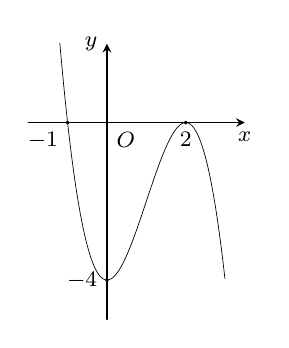
\begin{tikzpicture}[smooth,samples=300,scale=1,>=stealth,font=\footnotesize,line join=round, line cap=round, xscale=0.5, yscale=0.5]
	\def\xmin{-2} \def\xmax{3.5} \def\ymin{-5} \def\ymax{2} 
	\draw[->] (\xmin,0)--(0,0) node[below right]{$O$} -- (\xmax,0) node [below]{$x$};
	\draw[->] (0,\ymin)--(0,\ymax) node [left]{$y$};
	\clip (\xmin,\ymin) rectangle (\xmax,\ymax);
	\draw[line width=0.25, domain=-2:3,smooth]
	plot (\x,{-(\x)^3+3*(\x)^2-4});
	\draw[fill=black] (-1,0) circle(1pt) node[below left]{$-1$} (2,0) circle(1pt) node[below]{$2$} (0,-4) circle(1pt) node[left]{$-4$};
	\end{tikzpicture}	
	}
	\loigiai{
	Dựa vào đồ thị, hàm số $y=f(x)$ đạt giá trị cực đại là $0$ tại $x=2$.
	}
\end{ex}
%%==========Câu 10
\begin{ex}%[Đề 12 - Dự án đề VTED 2023 - Đợt 2 - Đoàn Minh Tân]%[2D2Y3-2]
	Cho $a>0$, $a\ne 1$, giá trị của $\log_a (4a)$ bằng
	\choice
	{$\dfrac{1}{4}\log_a 2$}
	{\True $2\log_a 2+1$}
	{$\dfrac{1}{2}\log_a 2+1$}
	{$4\log_a 2$}
	\loigiai{
	Ta có $\log_a (4a)=\log_a 4+\log_a a=2\log_a 2+1$.	
	}
\end{ex}

%%==========Câu 11
\begin{ex}%[2D1Y1-2]%Dự án tex đề Vted số 12%GV soạn Nguyễn Hữu Chung Kiên
	Hàm số $f(x)=x^3+a x^2+b x+c,$ $(a,$ $ b,$ $ c \in \mathbb{R})$ đồng biến trên $\mathbb{R}$ khi và chỉ khi
	\choice
	{ $f(x) \geq 0,$ $ \forall x \in \mathbb{R}$}
	{\True $f^{\prime}(x) \geq 0,$ $ \forall x \in \mathbb{R}$}
	{ $f(x)>0, $ $\forall x \in \mathbb{R}$}
	{ $f^{\prime}(x)>0,$ $ \forall x \in \mathbb{R}$}
	\loigiai{Ta có hàm số $y=f(x)$ đồng biến trên $\mathbb{R}$ khi và chỉ khi $f^{\prime}(x) \geq 0,$ $ \forall x \in \mathbb{R}$.
	}
\end{ex}
%%==========Câu 12
\begin{ex}%[2D3Y1-3]%Dự án tex đề Vted số 12%GV soạn Nguyễn Hữu Chung Kiên
	Cho hai hàm số $u(x),$ $ v(x)$ có đạo hàm liên tục trên $\mathbb{R}$. Khẳng định nào dưới đây đúng?
	\choice
	{\True $\displaystyle\int u(x) \cdot v^{\prime}(x) \mathrm{~d} x=u(x) \cdot v(x)-\displaystyle\int u^{\prime}(x) \cdot v(x) \mathrm{~d} x$}
	{ $\displaystyle\int u(x) \cdot v^{\prime}(x) \mathrm{~d} x=u(x) \cdot v(x)+\displaystyle\int u^{\prime}(x) \cdot v(x) \mathrm{~d} x$}
	{ $\displaystyle\int u(x) \cdot v^{\prime}(x) \mathrm{~d} x=u(x) \cdot v(x)-\displaystyle\int u^{\prime}(x) \cdot v^{\prime}(x) \mathrm{~d} x$}
	{ $\displaystyle\int u(x) \cdot v^{\prime}(x) \mathrm{~d} x=u(x) \cdot v(x)+\displaystyle\int u^{\prime}(x) \cdot v^{\prime}(x) \mathrm{~d} x $}
	\loigiai{Theo công thức nguyên hàm từng phần thì $$\displaystyle\int u(x) \cdot v^{\prime}(x) \mathrm{~d} x=u(x) \cdot v(x)-\displaystyle\int u^{\prime}(x) \cdot v(x) \mathrm{~d} x.$$
	}
\end{ex}
%%==========Câu 13
\begin{ex}%[2D3Y2-1]%Dự án tex đề Vted số 12%GV soạn Nguyễn Hữu Chung Kiên
	Nếu $\displaystyle\int\limits_2^3 f(x) \mathrm{~d} x=1$ thì $\displaystyle\int\limits_3^2 6 f(x) \mathrm{~d} x$ bằng
	\choice
	{ $6$}
	{\True $-6$}
	{ $\dfrac{1}{6}$}
	{ $-\dfrac{1}{6}$}
	\loigiai{Ta có $$\displaystyle\int\limits_3^2 6 f(x) \mathrm{~d} x =6\displaystyle\int\limits_3^2 f(x) \mathrm{~d} x=6\cdot \left(-\displaystyle\int\limits_2^3 f(x) \mathrm{~d} x\right)=6\cdot (-1)=-6.$$
	}
\end{ex}
%%==========Câu 14
\begin{ex}%[2D1B4-2]%Dự án tex đề Vted số 12%GV soạn Nguyễn Hữu Chung Kiên
	Tiệm cận đứng của đồ thị hàm số $y=\dfrac{2 x+1}{a x+1},$ $(a \in \mathbb{R} ;$ $ a \neq 0)$ là đường thẳng $x=1$ khi
	\choice
	{$a=1$}
	{ $a=-2$}
	{ $a=2$}
	{\True $a=-1$}
	\loigiai{Tiệm cận đứng của đồ thị hàm số $y=\dfrac{2 x+1}{a x+1},$ $(a \in \mathbb{R} ;$ $ a \neq 0)$ là đường thẳng $x=-\dfrac{1}{a}$.\\
	Ta cần $-\dfrac{1}{a}=1\Leftrightarrow a=-1.$
	}
\end{ex}
%%==========Câu 15
\begin{ex}%[2D3Y2-1]%Dự án tex đề Vted số 12%GV soạn Nguyễn Hữu Chung Kiên
	Nếu $\displaystyle\int\limits_1^2 f(x) \mathrm{~d} x=3$ và $\displaystyle\int\limits_1^2 g(x) \mathrm{~d} x=-1$ thì $\displaystyle\int\limits_1^2[2 f(x)+3 g(x)] \mathrm{~d} x$ bằng
	\choice
	{$2$}
	{$0$}
	{ $9$}
	{\True$3$}
	\loigiai{Ta có $$\displaystyle\int\limits_1^2[2 f(x)+3 g(x)] \mathrm{~d} x=2\displaystyle\int\limits_1^2 f(x) \mathrm{~d} x+3\displaystyle\int\limits_1^2 g(x) \mathrm{~d} x=2\cdot 3+3\cdot(-1)=3.$$
	}
\end{ex}
%%==========Câu 16
\begin{ex}%[2D1B1-1]%Dự án tex đề Vted số 12%GV soạn Nguyễn Hữu Chung Kiên
	Hàm số nào trong các hàm số sau nghịch biến trên $\mathbb{R}$? 
	\choice
	{\True $y=-x^3-3 x+4$}
	{ $y=1-x^4$}
	{ $y=-x^2+2$}
	{ $y=\dfrac{x+1}{x-2}$}
	\loigiai{
	\begin{itemize}
	\item Hàm số $y=-x^3-3 x+4$ có $y^\prime=-3x^2-3<0,$ $\forall x\in \mathbb{R}$ nên nghịch biến trên $\mathbb{R}$.
	\item Hàm số $y=1-x^4$ là hàm trùng phương nên không nghịch biến trên $\mathbb{R}$.
	\item Hàm số $y=-x^2+2$ là parabol nên không nghịch biến trên $\mathbb{R}$.
	\item Hàm số $y=\dfrac{x+1}{x-2}$ không xác định trên $\mathbb{R}$ nên không nghịch biến trên $\mathbb{R}$.
	\end{itemize}
	}
\end{ex}
%%==========Câu 17
\begin{ex}%[1D3B4-3]%Dự án tex đề Vted số 12%GV soạn Nguyễn Hữu Chung Kiên
	Biết ba số $3 ;$ $ x ;$ $ 15$ theo thứ tự lập thành một cấp số cộng. Tìm $x$?
	\choice
	{$x=3 \sqrt{5}$}
	{\True $x=9$}
	{ $x=12$}
	{ $x=6$}
	\loigiai{Vì ba số $3 ;$ $ x ;$ $ 15$ theo thứ tự lập thành một cấp số cộng nên ta có $2x=3+15\Leftrightarrow x=9.$
	}
\end{ex}
%%==========Câu 18
\begin{ex}%[2H2B2-1]%Dự án tex đề Vted số 12%GV soạn Nguyễn Hữu Chung Kiên
	Thể tích của khối cầu đường kính bằng $6$ là
	\choice
	{$48 \pi$}
	{ $36 \pi$}
	{ $144 \pi$}
	{\True $288 \pi$}
	\loigiai{Thể tích của khối cầu có bán kính $R$ là $V=\dfrac{4}{3}\pi R^3.$\\Đường kính bằng $6$ nên bán kính $R=\dfrac{6}{2}=3$.\\
	Vậy thể tích của khối cầu là $V=\dfrac{4}{3}\pi R^3=\dfrac{4}{3}\pi\cdot 6^3=288 \pi.$
	}
\end{ex}
%%==========Câu 19
\begin{ex}%[2D4B2-2]%Dự án tex đề Vted số 12%GV soạn Nguyễn Hữu Chung Kiên
	Phần thực của số phức $z=(2+3 i)\cdot (1-i)$ bằng
	\choice
	{$-5$}
	{\True $5$}
	{$1$}
	{$-1$}
	\loigiai{Ta có $z=(2+3 i)\cdot (1-i)=5+i.$\\
	Vậy phần thực của số phức $z=(2+3 i)\cdot (1-i)$ bằng $5$.
	}
\end{ex}
%%==========Câu 20
\begin{ex}%[2D2B5-2]%Dự án tex đề Vted số 12%GV soạn Nguyễn Hữu Chung Kiên
	Số nghiệm của phương trình $4^{x^2+3 x}=16$ là
	\choice
	{$3$}
	{\True $2$}
	{$0$}
	{$1$}
	\loigiai{Ta có $$4^{x^2+3 x}=16\Leftrightarrow 4^{x^2+3 x}=4^2\Leftrightarrow x^2+3 x=2\Leftrightarrow x^2+3 x-2=0\Leftrightarrow \hoac{&x=\dfrac{-3+\sqrt{17}}{2}\\&x=\dfrac{-3-\sqrt{17}}{2}.}$$
	Vậy phương trình $4^{x^2+3 x}=16$ có hai nghiệm.
	}
\end{ex}
%Nguyen Chien Thang(21-30)

%%==========Câu 21
\begin{ex}%[Dự án Đề thi thử Vted 12 Năm 2023-Lần 2]%[Nguyễn Chiến Thắng]%[2H1Y3-2]
	Công thức tính thể tích của khối lăng trụ có diện tích đáy $B$ và chiều cao $h$ là
	\choice
	{\True $V=B \cdot h$}
	{$V=\dfrac{1}{3} \cdot B \cdot h$}
	{$V=\dfrac{1}{2} \cdot B \cdot h$}
	{$V=3 \cdot B \cdot h$}
	\loigiai{Thể tích của khối lăng trụ có diện tích đáy $B$ và chiều cao $h$ là $V=B \cdot h$.
	}
\end{ex}

%%==========Câu 22
\begin{ex}%[Dự án Đề thi thử Vted 12 Năm 2023-Lần 2]%[Nguyễn Chiến Thắng]%[2D1B2-1]
	Số điểm cực trị của hàm số $y=(x-1)^2(x-2)$ là
	\choice
	{$3$}
	{\True $2$}
	{$ 1 $}
	{$0 $}
	\loigiai{Ta có $y'=2(x-1)(x-2)+(x-1)^2=3x^2-8x+5$. Suy ra $y'=0\Leftrightarrow \hoac{&x=1\\&x=\dfrac{5}{3}.}$\\ Bảng biến thiên
	\begin{center}
	
\begin{tikzpicture}[>=stealth]
	\tkzTabInit[nocadre=false,lgt=1,espcl=2,deltacl=0.5]{$x$/1 ,$y'$/.7,$y$/2}
	{$-\infty$ , $1$ , $\dfrac{5}{3}$ , $+\infty$}
	\tkzTabLine{ , + , $0$ , - , $0$ , + , }
	\tkzTabVar{-/$-\infty$ , +/$0$ , -/$-\dfrac{4}{27}$ , +/$+\infty$}
	\end{tikzpicture}
	\end{center}
	Vậy hàm số có hai điểm cực trị.
	}
\end{ex}

%%==========Câu 23
\begin{ex}%[Dự án Đề thi thử Vted 12 Năm 2023-Lần 2]%[Nguyễn Chiến Thắng]%[2D1B5-1]
	\immini{Đồ thị của hàm số nào dưới đây có dạng như đường cong trong hình bên?}
	{
	\begin{tikzpicture}[x=1cm,y=1cm,scale=0.6,>=stealth]
	\def\aa{-1} \def\bb{1} \def\cc{1} \def\dd{-2}
	\draw[->] (-4,0)--(6,0)node[below right]{$x$};
	\draw[->] (0,-5)--(0,4)node[left]{$y$};
	\fill (0,0)node[above left]{$O$};
	\draw[thin, dashed] (-4,-1)--(6,-1) (2,-5)--(2,4);
	\draw[black,samples=150,smooth,domain=-4:1.80] plot(\x,{(\aa*\x+\bb)/(\cc*\x+\dd)});
	\draw[black,samples=150,smooth,domain=2.25:6] plot(\x,{(\aa*\x+\bb)/(\cc*\x+\dd)});
	\path (2,0)coordinate[label=above right:$2$](A) (0,-1)coordinate[label=below left:$-1$](B) ;
	\foreach \diem in {A,B}\fill (\diem)circle(1.5pt);
	\end{tikzpicture}	
	}
	\choice
	{$y=x^3-4x^2+5$}
	{ $y=-x^3+4x^2-5$}
	{ $y=\dfrac{x-1}{x+2}$}
	{ \True $y=\dfrac{1-x}{x-2}$}
	\loigiai{ Đồ thị có hai tiệm cận là $x=2$ và $y=-1$ nên hàm số thỏa mãn là $y=\dfrac{1-x}{x-2}$.
	}
\end{ex}

%%==========Câu 24
\begin{ex}%[Dự án Đề thi thử Vted 12 Năm 2023-Lần 2]%[Nguyễn Chiến Thắng]%[1D2B2-1]
	Số cách lập một số tự nhiên gồm $2$ chữ số đều khác $0$ là
	\choice
	{$9 \cdot2$}
	{ $\mathrm{A}_9^2$}
	{ $\mathrm{C}_9^2$}
	{ \True $9^2$}
	\loigiai{ Gọi số cần lập là $\overline{ab}$, với $a,b\in\{1;2;3;\cdots;9\}$.\\
	Số cách chọn $a$ là $9$, và với mỗi cách chọn $a$ có $9$ cách chọn $b$.\\
	Vậy có $9^2$ số tự nhiên gồm $2$ chữ số đều khác $0$.
	}
\end{ex}

%%==========Câu 25
\begin{ex}%[Dự án Đề thi thử Vted 12 Năm 2023-Lần 2]%[Nguyễn Chiến Thắng]%[2H3B1-3]
	Trong không gian $Oxyz$, phương trình của mặt cầu tâm $I(1;-2;2)$ và bán kính $r=3$ là
	\choice
	{$(x+1)^2+(y-2)^2+(z+2)^2=3$}
	{ $(x+1)^2+(y-2)^2+(z+2)^2=9$}
	{ $(x-1)^2+(y+2)^2+(z-2)^2=3$}
	{ \True $(x-1)^2+(y+2)^2+(z-2)^2=9$}
	\loigiai{ Phương trình mặt cầu có tâm $I(a;b;c)$ bán kính $R$ là $(x-a)^2+(y-b)^2+(z-c)^2=R^2$.\\
	Vậy, phương trình thỏa mãn yêu cầu bài toán là $(x-1)^2+(y+2)^2+(z-2)^2=9$.
	}
\end{ex}

%%==========Câu 26
\begin{ex}%[Dự án Đề thi thử Vted 12 Năm 2023-Lần 2]%[Nguyễn Chiến Thắng]%[2H3Y2-2]
	Trong không gian $Oxyz$, một véc-tơ pháp tuyến của mặt phẳng $(P):2x-y+3z-4=0$ là
	\choice
	{ \True $\overrightarrow{n}_4=(2;-1;3)$}
	{ $\overrightarrow{n}_3=(2;1;3)$}
	{ $\overrightarrow{n}_2=(-2;-1;3)$}
	{ $\overrightarrow{n}_1=(2;-1;-3)$}
	\loigiai{Một véc-tơ pháp tuyến của $(P)$ là $\overrightarrow{n}_4=(2;-1;3)$.
	}
\end{ex}

%%==========Câu 27
\begin{ex}%[Dự án Đề thi thử Vted 12 Năm 2023-Lần 2]%[Nguyễn Chiến Thắng]%[2H3Y1-1]
	Trong không gian $Oxyz$, cho hai véc-tơ $\vec{u}=(1 ;-3 ; 2)$ và $\vec{v}=2 \vec{k}-2 \vec{i}-\vec{j}$. Tọa độ của véc-tơ $\vec{u}-2\vec{v}$ là
	\choice
	{\True $(5 ;-1 ;-2)$}
	{ $(-3 ;-5 ; 6)$}
	{ $(-3 ; 1 ; 4)$}
	{ $(5 ;-1 ; 6)$}
	\loigiai{Ta có $\vec{v}=(-2;-1;2) $ suy ra 
	$\vec{u}-2 \vec{v}=(5;-1;-2)$.
	}
\end{ex}

%%==========Câu 28
\begin{ex}%[Dự án Đề thi thử Vted 12 Năm 2023-Lần 2]%[Nguyễn Chiến Thắng]%[2D4Y1-1]
	Số phức liên hợp của số phức $z=1-2i$ là
	\choice
	{\True $\bar{z}=1+2 i$}
	{ $\bar{z}=-1-2 i$}
	{ $\bar{z}=-1+2 i$}
	{ $\bar{z}=-2+i$}
	\loigiai{Số phức liên hợp của số phức $z=1-2 i$ là $\bar{z}=1+2 i$.
	}
\end{ex}

%%==========Câu 29
\begin{ex}%[Dự án Đề thi thử Vted 12 Năm 2023-Lần 2]%[Nguyễn Chiến Thắng]%[2D3B1-1]
	Biết $F(x)$ là một nguyên hàm của hàm số $f(x)$ trên $\mathbb{R}$. Trong các khẳng định sau, khẳng định nào đúng?
	\choice
	{ $\displaystyle\int\limits[3f(x)-1] \mathrm{d}x=3F(x)-1+C$}
	{ $\displaystyle\int\limits[3f(x)-1] \mathrm{d}x=3xF(x)-1+C$}
	{ $\displaystyle\int\limits[3f(x)-1] \mathrm{d}x=3xF(x)-x+C$}
	{ \True$\displaystyle\int\limits[3f(x)-1] \mathrm{d}x=3F(x)-x+C$}
	\loigiai{Ta có $\displaystyle\int\limits[3f(x)-1] \mathrm{d}x=3\displaystyle\int\limits f(x)\mathrm{d}x-\displaystyle\int\limits \mathrm{d}x=3F(x)-x+C$
	}
\end{ex}

%%==========Câu 30
\begin{ex}%[Dự án Đề thi thử Vted 12 Năm 2023-Lần 2]%[Nguyễn Chiến Thắng]%[2H3B3-2]
	Trong không gian $O x y z$, cho hai điểm $M(1;1;2), N(0;3;3)$. Phương trình tham số của đường thẳng đi qua hai điểm $M, N$ là
	\choice
	{\True $\heva{&x=1+t \\& y=1-2 t \\& z=2-t}$}
	{$\heva{&x=-1+t \\& y=-1-2 t \\& z=-2-t}$}
	{ $\heva{&x=1+t \\& y=-2+t \\& z=-1+2 t}$}
	{ $ \heva{& x=1+t \\& y=1+t \\& z=2+t}$}
	\loigiai{Ta có $\vec{MN}=(-1;2;1)$. Chọn $\vec{u}=(1;-2;-1)$ làm một véc-tơ chỉ phương cho $MN$.\\
	Vậy, phương trình tham số của $MN$ là $\heva{&x=1+t \\& y=1-2 t \\& z=2-t.}$
	}
\end{ex}
%Lương Như Quỳnh(31-40)

%%==========Câu 31
\begin{ex}%[Lương Như Quỳnh]%[Tex hóa Đề Vted 2023]%[2D1B3-1]
	Biết hàm số $y=\dfrac{1}{3} x^3-3 x+2$ đạt giá trị nhỏ nhất trên $[1;3]$ bằng $m$ tại điểm $x_0$. Tổng $m+2 x_0$ bằng
	\choice
	{\True $2$}
	{$\dfrac{4}{3}$}
	{$8$}
	{$4-3 \sqrt{3}$}
	\loigiai{
	Ta có $ y'=x^2-3 $; $ y'=0\Leftrightarrow \hoac{&x=-\sqrt{3}&\not\in [1;3]&\\&x=\sqrt{3}&\in [1;3]&.}$\\
	Hàm số đã cho liên tục trên $ [1;3] $ và $ y(1)=-\dfrac{2}{3} $, $ y(3)=2 $, $ y\left(\sqrt{3}\right)=2-2\sqrt{3}$.\\
	Suy ra $ \min\limits_{[1;3]} y=2-2\sqrt{3}$ đạt tại $ x_0=\sqrt{3} $.\\
	Vậy $m+2 x_0=2-2\sqrt{3}+2\sqrt{3}=2$.
	}
\end{ex}

%%==========Câu 32
\begin{ex}%[Lương Như Quỳnh]%[Tex hóa Đề Vted 2023]%[2D2B6-2]
	Tổng các nghiệm nguyên của bất phương trình $\log _2(2 x+3)<\log _2(10-x)$ bằng
	\choice
	{$5$}
	{$3$}
	{\True $2$}
	{$4$}
	\loigiai{
	Ta có 
	\[ \log _2(2 x+3)<\log _2(10-x) 
	\Leftrightarrow \heva{&2 x+3>0\\&2 x+3<10-x} 
	\Leftrightarrow -\dfrac{3}{2}<x<\dfrac{7}{3}.\]
	Vì $ x $ nguyên nên $ x\in \{-1;0;1;2\} $.\\
	Vậy tổng các nghiệm nguyên của bất phương trình đã cho là $ -1+0+1+2=2 $.
	}
\end{ex}

%%==========Câu 33
\begin{ex}%[Lương Như Quỳnh]%[Tex hóa Đề Vted 2023]%[1H3B4-3]
	Cho hình chóp tứ giác đều có tất cả các cạnh bằng $a$. Cô-sin góc giữa mặt bên và mặt đáy của hình chóp đã cho bằng
	\choice
	{$\dfrac{1}{4 \sqrt{3}}$}
	{$\dfrac{1}{4 \sqrt{2}}$}
	{\True $\dfrac{1}{\sqrt{3}}$}
	{$\dfrac{1}{\sqrt{2}}$}
	\loigiai{
	\immini{
	Gọi $ O $ là tâm của hình vuông $ ABCD $, $ M $ là trung điểm $ CD $.\\
	Ta có $ \heva{&CD\perp OM\\
	&CD\perp SO} $ suy ra $ CD\perp(SOM) $.\\
	Ta có $ \heva{&(SCD)\cap (ABCD)=CD\\&(SOM)\perp CD\\
	&(SOM)\cap (SCD)=SM\\&(SOM)\cap (ABCD)=OM} $ \\suy ra $ ((SCD),(ABCD))=(SM, OM)=\widehat{SMO} $.\\
	Xét tam giác $ SOM $ vuông tại $ O $, ta có $ \cos \widehat{SMO}=\dfrac{OM}{SM}=\dfrac{\dfrac{a}{2}}{\dfrac{a\sqrt{3}}{2}}=\dfrac{1}{\sqrt{3}}$.
	}
	{
	\begin{tikzpicture}[font=\footnotesize,line cap=round,line join=round, >=stealth,scale=0.7]
	\def \a{-2} \def \b{-1}\def \c{5} \def \h{4} 
	\path (.5,.5)coordinate(A) 	
	+(\a,\b)coordinate(B)
	+(\c,0)coordinate(D)
	($(B)+(D)-(A)$)coordinate(C);
	\path ($(C)!1/2!(A)$)coordinate(O);
	\path ($(C)!1/2!(D)$)coordinate(M);
	\coordinate (S)at ($(O)+(0,\h)$);
	\draw [dashed] (D)--(A)--(C) (D)--(B)--(A)--(S)--(O)--(M);
	\draw (S)--(D)--(C)--(S)--(C)--(B)--
	(S)--(M);	
	\foreach \x/\g in{A/160,D/0, C/-90,B/-90, S/90, O/-90, M/-45}
	\fill[black](\x) circle (1pt)($(\x)+(\g:3.5mm)$) node{\small $\x$};
	\foreach \x/\o/\y/\r in {S/O/M/2} \draw ($(\o)!\r mm!(\x)$)--($($(\o)!\r mm!(\x)$)+($(\o)!\r mm!(\y)$)-(\o)$)--($(\o)!\r mm!(\y)$);
	%\draw[-] ($(M)!6mm!(S)$) to[bend right=45] node[pos=.5,left]{$\varphi$} ($(M)!6mm!(O)$);	
	\draw[-] ($(M)!5mm!(S)$) to[bend right=45] ($(M)!5mm!(O)$);	
	\end{tikzpicture}
	}
	}
\end{ex}

%%==========Câu 34
\begin{ex}%[Lương Như Quỳnh]%[Tex hóa Đề Vted 2023]%[2H3B2-3]
	Trong không gian $Oxyz$, cho hai điểm $A(-1;0;2)$, $B(3;2;0)$. Phương trình mặt phẳng trung trực của $AB$ là
	\choice
	{$x+y+z+2=0$}
	{$2 x+y-z+2=0$}
	{$x+y+z-2=0$}
	{\True $2x+y-z-2=0$}
	\loigiai{
	Ta có $\overrightarrow{AB}=(4;2;-2)=2(2;1;-1)$.\\
	Gọi $(P)$ là mặt phẳng trung trực của $AB$. Ta có phương trình $(P)$ đi qua trung điểm $I(1;1;1)$ của $AB$ và nhận $\overrightarrow{n}=(2;1;-1) $ làm một véc-tơ pháp tuyến là
	\[(P)\colon 2(x-1)+(y-1)-(z-1)=0\Leftrightarrow 2x+y-z-2=0.\]
	}
\end{ex}

%%==========Câu 35
\begin{ex}%[Lương Như Quỳnh]%[Tex hóa Đề Vted 2023]%[2D4B4-1]
	Xét hai số thực $a$, $b$ sao cho phương trình $z^2+az+b=0$ có một nghiệm phức $1-i$. Nghiệm phức còn lại của phương trình trên là
	\choice
	{$-1-i$}
	{$1-i$}
	{$-1+i$}
	{\True $1+i$}
	\loigiai{
	Xét phương trình $z^2+az+b=0$ với $a$, $b$ là hai số thực.\\
	Vì phương trình có một nghiệm phức $z=1-i$ nên $z=1+i$ cũng là một nghiệm.
	}
\end{ex}

%%==========Câu 36
\begin{ex}%[Lương Như Quỳnh]%[Tex hóa Đề Vted 2023]%[1H3B5-3]
	Cho khối chóp $S.ABCD$ có đáy $ABCD$ là hình thoi tâm $O$, $AC=2a$, $BD=2\sqrt{3} a$, $SO\perp(ABCD)$ và $SO=\sqrt{6} a$. Khoảng cách từ điểm $O$ đến mặt phẳng $(SBC)$ bằng
	\choice
	{$\dfrac{\sqrt{6} a}{3}$}
	{\True $\dfrac{\sqrt{3} a}{2}$}
	{$\dfrac{a}{2}$}
	{$\dfrac{\sqrt{6} a}{2}$}
	\loigiai{
	\immini{
	Gọi $ M $ là trung điểm $ BC $. \\
	Kẻ đường cao $ OH $ của tam giác $ SOM $ vuông tại $ O $.\\
	Ta có $ \heva{&BC\perp OM\\
	&BC\perp SO} $ suy ra $ BC\perp (SOM) $.\\
	Ta có $ \heva{&OH \perp BC} $ suy ra $ OH \perp (SBC)$.\\
	Do đó $ OH=\mathrm{d}(O,(SBC)) $.\\
	Xét tam giác $OBC$ vuông tại $ O $, ta có \[BC=\sqrt{OB^2+OC^2}=\sqrt{\left(\sqrt{3}a\right)^2+a^2}=2a.\]
	Lại có $OM\cdot BC=OC\cdot OC\Rightarrow OM=\dfrac{OB\cdot OC}{BC}=\dfrac{\sqrt{3}a\cdot a}{2a}=\dfrac{\sqrt{3} a}{2}$.
	}
	{
	\begin{tikzpicture}[font=\footnotesize,line cap=round,line join=round, >=stealth,scale=0.7]
	\def \a{-2} \def \b{-1}\def \c{5} \def \h{4} 
	\path (.5,.5)coordinate(A) 	
	+(\a,\b)coordinate(B)
	+(\c,0)coordinate(D)
	($(B)+(D)-(A)$)coordinate(C);
	\path ($(C)!1/2!(A)$)coordinate(O);
	\path ($(B)!3/7!(C)$)coordinate(M);
	\path ($(S)!3/5!(M)$)coordinate(H);
	\coordinate (S)at ($(O)+(0,\h)$);
	\draw [dashed] (D)--(A)--(C) (D)--(B)--(A)--(S)--(O)--(M) (O)--(H);
	\draw (S)--(D)--(C)--(S)--(C)--(B)--
	(S)--(M);	
	\foreach \x/\g in{A/160,D/0, C/-90,B/-90, H/0, S/90, O/-90, M/-45}
	\fill[black](\x) circle (1pt)($(\x)+(\g:2.5mm)$) node{\small $\x$};
	\foreach \x/\o/\y/\r in {M/O/S/2,O/M/C/3,M/H/O/2} \draw ($(\o)!\r mm!(\x)$)--($($(\o)!\r mm!(\x)$)+($(\o)!\r mm!(\y)$)-(\o)$)--($(\o)!\r mm!(\y)$);
	\end{tikzpicture}
	}
	}
\end{ex}

%%==========Câu 37
\begin{ex}%[Lương Như Quỳnh]%[Tex hóa Đề Vted 2023]%[1D2B5-2]
	Trong $100$ số nguyên dương đầu tiên, xác suất để chọn được một số chia hết cho $8$ bằng
	\choice
	{$\dfrac{9}{100}$}
	{$\dfrac{1}{10}$}
	{\True $\dfrac{3}{25}$}
	{$\dfrac{11}{100}$}
	\loigiai{
	Trong $100$ số nguyên dương đầu tiên, có $ 12 $ số chia hết cho $8$, bao gồm $ \{8;16;24;\ldots;80;88;96\} $.\\
	Vậy xác suất cần tìm là $ \mathrm{P}=\dfrac{12}{100}= \dfrac{3}{25}$.
	}
\end{ex}

%%==========Câu 38
\begin{ex}%[Lương Như Quỳnh]%[Tex hóa Đề Vted 2023]%[2D2B3-2]
	Xét hai số thực dương $a$, $b$ thay đổi thỏa mãn $3 \log _3 a+2 \log _3 \sqrt{b}=1$, khẳng định nào sau đây đúng?
	\choice
	{$a^3=3 b$}
	{$a^3 b=1$}
	{\True $a^3 b=3$}
	{$a^3 b^2=3$}
	\loigiai{
	Với $a$, $b$ là hai số thực dương, ta có 
	\[3 \log _3 a+2 \log _3 \sqrt{b}=1\Leftrightarrow \log _3 a^3+ \log _3 b=1\Leftrightarrow \log _3 a^3b=1 \Leftrightarrow a^3b=3.\]
	}
\end{ex}

%%==========Câu 39
\begin{ex}%[Lương Như Quỳnh]%[Tex hóa Đề Vted 2023]%[2D2B5-3]
	Tổng các nghiệm của phương trình $\left(2^{x+3}-1\right) \sqrt{-\log _2^2 x+5 \log _2 x-4}=0$ là
	\choice
	{$15$}
	{\True $18$}
	{$2$}
	{$5$}
	\loigiai{
	Ta có 
	\allowdisplaybreaks
	\begin{eqnarray*}
	&& \left(2^{x+3}-1\right) \sqrt{-\log _2^2 x+5 \log _2 x-4}=0 \\ 
	&\Leftrightarrow& \heva{& x>0\\&\hoac{&2^{x+3}-1=0\\&-\log _2^2 x+5 \log _2 x-4=0}} 
	\Leftrightarrow \heva{& x>0\\&\hoac{&x+3=0\\&\log _2 x=1\\&\log _2x =4}}\\ 
	&\Leftrightarrow& \heva{& x>0\\&\hoac{&x=-3\\&x=2\\&x=16.}\Leftrightarrow \hoac{&x=2\\&x=16.}}
	\end{eqnarray*}
	Vậy tổng các nghiệm của phương trình đã cho là $ 2+16=18 $.
	}
\end{ex}

%%==========Câu 40
\begin{ex}%[Lương Như Quỳnh]%[Tex hóa Đề Vted 2023]%[2D1B5-3]
	Cho hàm số $f(x)$ có bảng biến thiên như sau
	\begin{center}
	
\begin{tikzpicture}
	\tkzTabInit[nocadre=false,lgt=1.2,espcl=2.5,deltacl=0.6]
	{$x$ /0.6, $y'$ /0.6, $y$ /2.}
	{$-\infty$,$0$,$2$,$+\infty$}
	\tkzTabLine{,-,$0$,+,$0$,-,}
	\tkzTabVar{+/$+\infty$,-/$1$,+/$5$,-/$-\infty$}
	\end{tikzpicture}
	\end{center}
	Xét $g(x)=f^2(x)-4 f(x)$. Số nghiệm thực phân biệt của phương trình $g'(x)=0$ là
	\choice
	{\True $5$}
	{$4$}
	{$6$}
	{$3$}
	\loigiai{
	Ta có $g'(x)=2f(x)\cdot f'(x)-4 f'(x)=2f'(x)\left[f(x)-2\right]$.\\
	$g'(x)=0\Leftrightarrow \hoac{&f'(x)=0\\&f(x)=2}\Leftrightarrow \hoac{&x=0\\&x=2\\&x=a \quad(a<0)\\&x=b\quad(0<b<2)\\&x=c\quad(c>2).\\}$\\
	Vậy phương trình $g'(x)=0$ có $ 5 $ nghiệm thực phân biệt.
	}
\end{ex}
%Loc Do(41-44)

%%==========Câu 41
\begin{ex}%[Loc Do]%[Tex hóa Đề Vted 2023]%[2H3G3-2]
	Trong không gian $Oxyz$, cho đường thẳng $d\colon \heva{&x=1+2t\\&y=1-t\\&z=1+2t}$ và đường thẳng $d'$ qua điểm $A(1;1;1)$ có một véc-tơ chỉ phương $\vec{u}=(1;1;4)$. Đường thẳng qua $M(2;3;7)$ cắt $d$, $d'$ lần lượt tại $B$ và $C$ sao cho $A$, $B$, $C$ là ba đỉnh của tam giác cân tại $B$ có phương trình là
	\choice
	{\True $\dfrac{x-2}{1}=\dfrac{y-3}{-3}=\dfrac{z-7}{-1}$}
	{$\dfrac{x-2}{1}=\dfrac{y-3}{-6}=\dfrac{z-7}{-4}$}
	{$\dfrac{x-2}{1}=\dfrac{y-3}{2}=\dfrac{z-7}{6}$}
	{$\dfrac{x-2}{1}=\dfrac{y-3}{-2}=\dfrac{z-7}{-2}$}
	\loigiai{
	\textbf{Cách 1:}
	Ta có $d\cap d' =A(1;1;1)$. Vì $BA=BC \Rightarrow \widehat{BCA}=\widehat{BAC}=(d,d')=45^\circ$, $\left(\cos (d,d') = \dfrac{|\overrightarrow{u}_d\cdot \overrightarrow{u}_{d'}|}{|\overrightarrow{u}_d|\cdot |\overrightarrow{u}_{d'}|}=\dfrac{1}{\sqrt{2}}\right)$.
	\begin{center}
	\begin{tikzpicture}[>=stealth,line join=round,line cap=round,font=\footnotesize,scale=1]
	\coordinate (B)at(0,0);
	\coordinate (A)at(3,0);
	\coordinate (C)at(0,3);
	\coordinate (M)at(0,-1);
	\draw (-0.5,0)--(4,0) node [above] {$d$};
	\draw (0,-1)--(0,3.5) ;
	\draw (-0.2,3.2)--(3.2,-0.2) node [right] {$d'$};
	\path pic[angle radius=2mm,draw=blue] {right angle = A--B--C};
	\path pic[angle radius=3mm,draw=blue,fill=green!40,"$45^\circ$",angle eccentricity=2.5] { angle = C--A--B};
	\foreach \i/\g in {A/60,C/30,B/-120,M/-90}{\draw[fill=black](\i) circle (1.0pt) ($(\i)+(\g:3mm)$) node[scale=1]{$\i$};}
	\end{tikzpicture}
	\end{center}
	Suy ra $\widehat{ABC}=90^\circ \Rightarrow MB\perp d$. Gọi $B(2b+1;-b+1;2b+1)\in d$. \\
	Ta có $\overrightarrow{MB}=\left(2b-1;-b-2;2b-6\right);\, \overrightarrow{u}_d=(2;-1;2)$.
	\[
	\overrightarrow{MB} \perp \overrightarrow{u}_d \Leftrightarrow 2(2b-1)+b+2+2(2b-6) =0 \Leftrightarrow b=\dfrac{4}{3}.
	\]
	Suy ra $\overrightarrow{MB}=\left(\dfrac{5}{3};-\dfrac{10}{3};-\dfrac{10}{3}\right) =\dfrac{5}{3} (1;-2;-2) \Rightarrow MB:\dfrac{x-2}{1}=\dfrac{y-3}{-2}=\dfrac{z-7}{-2}$.\\
	\textbf{Cách 2:} Ta có $d':\heva{
	&x=1+t\\
	&y=1+t\\
	&z=1+4t.
	}$ \\
	Gọi $B\left(2b+1;-b+1;2b+1\right)\in d; C(c+1;c+1;4c+1)\in d'$, $(B\neq A; C\neq A \Rightarrow b,c\neq 0)$.
	\begin{eqnarray*}
	\text{Vì} \quad BA=BC &\Leftrightarrow & 9b^2=(2b-c)^2+(b+c)^2+(2b-4c)^2=9b^2+18c^2-18bc\\
	&\Leftrightarrow & 18c(c-b)=0 \Leftrightarrow b=c.
	\end{eqnarray*}
	\[ \Rightarrow \overrightarrow{u}_{\Delta} =\overrightarrow{BC}=(c-2b;c+b;4c-2b)=(-b;2b;2b) =-b(1;-2;-2).
	\]
	Suy ra $\Delta: \dfrac{x-2}{1}=\dfrac{y-3}{-2}=\dfrac{z-7}{-2}$.
	}
\end{ex}

%%==========Câu 42
\begin{ex}%[Loc Do]%[Tex hóa Đề Vted 2023]%[2H1K3-2]
	Cho khối chóp $S.ABC$ có đáy $ABC$ là tam giác đều cạnh $a$, $SA\perp (ABC)$, cô-sin của góc giữa hai mặt phẳng $(SAB)$ và $(SBC)$ bằng $\dfrac{1}{\sqrt{5}}$. Thể tích của khối chóp $S.ABC$ bằng
	\choice
	{$\dfrac{\sqrt{3}a^3}{4}$}
	{$\dfrac{\sqrt{2}a^3}{2}$}
	{$\dfrac{3\sqrt{3}a^3}{4}$}
	{\True $\dfrac{a^3}{4}$}
	\loigiai{
	Kẻ $CH\perp AB\Rightarrow CH\perp (SAB)\Rightarrow CH\perp SB$; kẻ $HK\perp SB \Rightarrow SB\perp (CHK) \Rightarrow \left((SAB),(SBC)\right)=\widehat{HKC}$.
	\begin{center}
	\begin{tikzpicture}[scale=1, font=\footnotesize, line join=round, line cap=round, >=stealth]
	\def\ac{5} % cạnh AC
	\def\ab{3} % cạnh AB
	\def\h{3} % chiều cao
	\def\gocA{40} % góc A của đáy
	\coordinate[label=left:$A$] (A) at (0,0);
	\coordinate[label=right:$B$] (B) at (\ac,0);
	\coordinate[label=below left:$C$] (C) at (-\gocA:\ab);
	\coordinate[label=above:$S$] (S) at ($(A)+(90:\h)$);
	\draw (A)--(C)--(B)--(S)--cycle (S)--(C);
	\draw[dashed] (A)--(B);
	\coordinate [label=above left:$H$] (H) at ($(A)!(C)!(B)$);
	\coordinate [label=above right:$K$] (K) at ($(S)!(H)!(B)$);
	\draw[dashed] (C)--(H)--(K);
	\path[,line width=0.6pt] pic[angle radius=2mm,draw=blue,fill=green!20] {right angle = H--K--B};
	\draw (C)--(K);
	\path[,line width=0.6pt] pic[angle radius=2mm,draw=blue,fill=green!20] {right angle = C--H--B};
	\foreach \diem in {A,B,C,S,H,K}	\fill (\diem)circle(1.5pt);
	\newcommand{\gocv}[4][black]{\draw[#1] ($(#3)!5pt!(#2)$)--($(#3)!2!($($(#3)!5pt!(#2)$)!.5!($(#3)!5pt!(#4)$)$)$)--($(#3)!5pt!(#4)$);}
	\gocv{S}{A}{C}
	\end{tikzpicture}
	\end{center}
	Ta có $\cos \widehat{HKC}=\dfrac{1}{\sqrt{5}}\Rightarrow \tan \widehat{HKC}=2 \Rightarrow \dfrac{HC}{HK}=2 \Rightarrow HK=\dfrac{1}{2}HC=\dfrac{\sqrt{3}a}{4}$.\\
	Suy ra $\sin \widehat{KBH}=\dfrac{HK}{HB}=\dfrac{\sqrt{3}}{2}\Rightarrow \widehat{KBH}=60^\circ \Rightarrow SA=AB\cdot \tan 60^\circ =\sqrt{3}a$.\\
	Vậy $V_{S.ABC}=\dfrac{1}{3}\cdot S_{ABC}\cdot SA = \dfrac{1}{3}\cdot \dfrac{\sqrt{3}a^2}{4}\cdot \sqrt{3}a = \dfrac{a^3}{4}$.
	}
\end{ex}

%%==========Câu 43
\begin{ex}%[Loc Do]%[Tex hóa Đề Vted 2023]%[2D4G5-1]
	Xét hai số phức $z$, $w$ thoả mãn $|z|=2$, $|w|=4$ và $(z-i)(\overline{w}+i)$ là số thuần ảo. Giá trị lớn nhất của $\left| z-w\right|$ bằng
	\choice
	{$2\sqrt{10}-1$}
	{\True $\sqrt{19}+1$}
	{$6$}
	{$3\sqrt{2}+1$}
	\loigiai{
	\immini{ Vì $|z|=2;|w| =4 \Rightarrow M(z)\in (C_1), N(w)\in (C_2)$ có cùng tâm $O(0;0)$ và bán kính $R_1=2; R_2=4$.
	Đặt $M(x;y), N(a;b) \Rightarrow (z-i)(\overline{w}+i)=(x+(y-1)i)(a+(1-b)i)$ là số thuần ảo khi phần thực bằng $0$ tức là
	\begin{eqnarray*}
	ax-(y-1)(1-b)=0 &\Leftrightarrow & xa+(y-1)(b-1)=0 \\
	&\Leftrightarrow & \overrightarrow{PM}\cdot \overrightarrow{PN}=0 \\
	&\Leftrightarrow & PM\perp PN
	\end{eqnarray*}}
	{
	\begin{tikzpicture}[scale=1, font=\footnotesize, line join=round, line cap=round, >=stealth, y=0.5cm,x=0.5cm]
	\coordinate (O)at(0,0);
	\coordinate (P)at(0,1);
	\draw[line width=0.6pt,black] (O) circle (1cm);
	\draw[line width=0.6pt,black] (O) circle (2cm);
	\coordinate (M) at ($(O)+(110:2)$);
	\coordinate (M_0) at ($(O)+(-20:2)$);
	\coordinate (N) at ($(O)+(190:4)$);
	\coordinate (N_0) at ($(O)+(240:4)$);
	\coordinate (E_0) at (intersection cs:first line={(P)--(O)}, second line={(M_0)--(N_0)});
	\coordinate (E) at ($(N)!.5!(M)$);	
	\path pic[angle radius=2mm,draw=blue,fill=green!20] {right angle = M--P--N};
	\path pic[angle radius=2mm,draw=blue,fill=green!20] {right angle = M_0--P--N_0};
	\draw (M)--(N) (P)--(M_0)--(N_0)--(P)--(E_0) (N)--(P)--(M) (E)--(P);
	\foreach \i/\g in {O/0,M/60,M_0/0,N/180,N_0/210,P/0,E_0/130,E/120}{\draw[fill=black](\i) circle (1pt) ($(\i)+(\g:3mm)$) node[scale=1]{$\i$};}	
	\end{tikzpicture}
	}
	\noindent
	Trong đó $P(0;1); \overrightarrow{PM}=(x;y-1); \overrightarrow{PN}=(a;b-1)$.\\
	Gọi $E$ là trung điểm $MN$ ta có $|z-w| =MN=t,(t>0)$\\
	Ta có $MN=2PE\leq 2(PO+OE)=2(1+OE)=2\left(1+\sqrt{\dfrac{2(OM^2+ON^2)-MN^2}{4}}\right)$.\\
	Suy ra
	\[
	t\leq 2\left(1+\sqrt{\dfrac{2(4+16)-t^2}{4}}\right) \Leftrightarrow t-2\leq\sqrt{40-t^2} \Leftrightarrow t\leq \sqrt{19}+1 \Rightarrow |z-w|_{\max} =\sqrt{19}+1.
	\]
	Dấu \lq\lq=\rq\rq\ xảy ra khi $P,O,E$ thẳng hàng theo thứ tự và $OE=\dfrac{\sqrt{19}+1}{2}-1=\dfrac{\sqrt{19}-1}{2}$ tức là $E\equiv E_0; M\equiv M_0; N\equiv N_0$.\\
	\textbf{\textit{Tìm giá trị nhỏ nhất:}} $MN=2PE \geq 2(OE-OP)=2(OE-1) =2\left(\sqrt{\dfrac{2(OM^2+ON^2)-MN^2}{4}}-1\right)$\\
	Suy ra $t\geq 2\left(\sqrt{\dfrac{2(4+16)-t^2}{4}}-1\right) \Rightarrow t\geq \sqrt{19}-1\Rightarrow |z-w|_{\min} =\sqrt{19}-1$.	}
\end{ex}

%%==========Câu 44
\begin{ex}%[Loc Do]%[Tex hóa Đề Vted 2023]%[2D3K2-1]
	Cho hàm số $f(x)$ có đạo hàm $f'(x)=\heva{&\mathrm{e}^x & ~\text{khi}~ x\ge 0\\&\mathrm{e}^{-x} & ~\text{khi}~ x<0}$. Gọi $F$ là một nguyên hàm của $f$ trên $\mathbb{R}$ sao cho $F(-1)+F(1)=1$, khi đó $F(-2)+F(2)$ bằng
	\choice
	{$2\mathrm{e}^2+2\mathrm{e}+1$}
	{\True $2\mathrm{e}^2-2\mathrm{e}-1$}
	{$2\mathrm{e}^2+2\mathrm{e}-1$}
	{$2\mathrm{e}^2-2\mathrm{e}+1$}
	\loigiai{
	\textbf{Cách 1:}
	Ta có $f(x) =\heva{
	&e^x+C_1\,\,\text{khi}\,\, x\geq 0\\
	&-e^{-x}+C_2\,\,\text{khi}\,\, x<0
	}$ vì có đạo hàm trên $\mathbb{R}$ $\left(f'(0^+)=f'(0^-)=1\right)$ nên $f(x)$ liên tục trên $\mathbb{R}$. Suy ra 
	\[\lim_{x\rightarrow 0^{+}} f(x)=\lim_{x\rightarrow 0^{-}} f(x)=f(0) \Leftrightarrow 1+C_1=-1+C_2\Rightarrow C_1-C_2=-2
	\]
	Khi đó
	\begin{eqnarray*} 
	F(-2)+F(2)&= &F(-1)+F(1)+\displaystyle\int\limits_1^2 f(x)dx +\displaystyle\int\limits_{-1}^{-2} f(x)dx\\
	&=& 1+\displaystyle\int\limits_1^2 (\mathrm{e}^x+C_1)dx-\displaystyle\int\limits_{-2}^{-1} (-\mathrm{e}^{-x}+C_2) dx\\
	&= &1+\displaystyle\int\limits_1^2 \mathrm{e}^x dx+\displaystyle\int\limits_{-2}^{-1} \mathrm{e}^{-x} dx+C_1\displaystyle\int\limits_1^2 dx-C_2\displaystyle\int\limits_{-2}^{-1} dx
	=2\mathrm{e}^2-2\mathrm{e}+1+C_1-C_2=2\mathrm{e}^2-2\mathrm{e}-1.
	\end{eqnarray*}
	\textbf{Cách 2:} Ta có $f(x) = \heva{
	&e^x+C_1\,\,\text{khi}\,\, x\geq 0\\
	&-e^{-x}+C_2\,\,\text{khi}\,\, x< 0
	}$ vì có đạo hàm trên $\mathbb{R}$ $\left(f'(0^+)=f'(0^-)=1\right)$ nên $f(x)$ liên tục trên $\mathbb{R}$. Suy ra 
	\[\lim_{x\rightarrow 0^{+}} f(x)=\lim_{x\rightarrow 0^{-}} f(x)=f(0) \Leftrightarrow 1+C_1=-1+C_2\Rightarrow C_1-C_2=-2.\]
	Suy ra
	\begin{eqnarray*}
	& &F(x)=\heva{
	&\mathrm{e}^x+C_1x+D_1\,\,\text{khi}\,\, x\geq 0\\
	&\mathrm{e}^{-x}+C_2x+D_2\,\,\text{khi}\,\, x<0.
	}\\
	&\Rightarrow& F(-1)+F(1)=2\mathrm{e}+C_1-C_2+D_1+D_2=2\mathrm{e}-2+D_1+D_2=1 \Leftrightarrow D_1+D_2=3-2\mathrm{e}\\
	&\Rightarrow & F(-2)+F(2)=2\mathrm{e}^2+2(C_1-C_2)+D_1+D_2=2\mathrm{e}^2-4+(3-2\mathrm{e})=2\mathrm{e}^2-2\mathrm{e}-1.
	\end{eqnarray*}
	}
\end{ex}
%Lee Van Toan(45-47)

%%==========Câu 45
\begin{ex}%[Lee Van Toan]%[Tex hóa Đề Vted 2023]%[2D4G3-4]
	Có bao nhiêu số phức $z$ mà phần thực và phần ảo đều là các số nguyên thuộc đoạn $[-10;10]$ sao cho $A$, $B$, $C$ lần lượt là điểm biểu diễn của các số phức $z$; $z+\dfrac{1}{z}$; $\dfrac{1}{z}$ thì $OABC$ là một hình chữ nhật?
	\choice
	{$20$}
	{$21$}
	{\True $40$}
	{$41$}
	\loigiai{
	Điều kiện $z \neq 0$.\\
	Đặt $z=x+yi$, $(x,\ y \in \mathbb{R}) \Rightarrow \dfrac{1}{z}=\dfrac{1}{x+yi}=\dfrac{x-yi}{x^2+y^2} \Rightarrow A(x;y)$, $B(x+a;y+b)$, $C(a;b)$ với $a=\dfrac{x}{x^2+y^2}$; $b=-\dfrac{y}{x^2+y^2}$.\\
	Khi đó $OABC$ là hình chữ nhật khi $OABC$ là hình bình hành và $\widehat{AOC}=90^\circ$ khi và chỉ khi
	$$ \heva{&\overrightarrow{OA}=\overrightarrow{CB} \\ &\overrightarrow{OA}\perp \overrightarrow{OC}} \Leftrightarrow ax+by=0 \Leftrightarrow x^2-y^2=0 \Leftrightarrow y= \pm x.$$
	\begin{itemize}
	\item Nếu $x=0 \Rightarrow y=0 \Rightarrow z=0$ (loại).
	\item Nếu $x \in\{-10, \ldots, 10\} \setminus \{0\}$ có $20$ cách chọn và $y= \pm x$ tương ứng có $2$ cách chọn nên có $40$ cặp $(x;y)$ tương ứng với $40$ số phức thoả mãn.
	\end{itemize}
	}
\end{ex}

%%==========Câu 46
\begin{ex}%[Lee Van Toan]%[Tex hóa Đề Vted 2023]%[2D3G3-1]
	Cho hàm số $f(x)=x^3+ax^2+bx+c$, ($a$, $b$, $c \in \mathbb{R}$) có đồ thị $(C)$. Biết rằng $f(x)$ có hai điểm cực trị $x_1$, $x_2$ thoả mãn $f\left(x_1\right)=f\left(x_2\right)+4$. Đường thẳng qua điểm $M\left(x_2;f\left(x_2\right)\right)$ cắt $(C)$ tại điểm thứ hai $N\left(x_0;f\left(x_2\right)\right)$. Gọi $y=g(x)$ là hàm số bậc hai có đồ thị qua $N$ và hai điểm cực trị của $(C)$. Diện tích hình phẳng giới hạn bởi hai đường $y=f(x)$ và $y=g(x)$ bằng
	\choice
	{$\dfrac{19}{4}$}
	{$\dfrac{25}{6}$}
	{$\dfrac{23}{4}$}
	{\True $\dfrac{37}{12}$}
	\loigiai{
	Ta có $f(x)-g(x)=x^3+\ldots$ có ba nghiệm $x_0$, $x_1$, $x_2$ nên $f(x)-g(x)=\left(x-x_0\right)\left(x-x_1\right)\left(x-x_2\right)$.\\
	Ta có $f'(x)=3x^2+2ax+b=3\left(x-x_1\right)\left(x-x_2\right)$.\\
	Do đó $f\left(x_2\right)-f\left(x_1\right)=\displaystyle\int\limits_{x_1}^{x_2}f'(x)\mathrm{\,d}x=\displaystyle\int\limits_{x_1}^{x_2} 3\left(x-x_1\right)\left(x-x_2\right)\mathrm{\,d}x=\dfrac{1}{2}\left(x_1-x_2\right)^3=-4 \Leftrightarrow x_2=x_1+2$.\\
	Vì $x_1$, $x_2$ là hai nghiệm của $f'(x)=0$ nên theo định lí vi-ét có $x_1+x_2=-\dfrac{2a}{3}$.\\
	Đường thẳng $MN \colon y=f\left(x_2\right)$ nên phương trình $f(x)-f\left(x_2\right)=x^3+ax^2+bx+c-f\left(x_2\right)$ có hai nghiệm $x_0$, $x_2$ (trong đó $x_2$ là nghiệm kép) và cũng theo định lí vi-ét có $$x_0+x_2+x_2=-a \Rightarrow x_0=\dfrac{3}{2}\left(x_1+x_2\right)-2 x_2=\dfrac{3 x_1-x_2}{2}=\dfrac{3 x_1-\left(x_1+2\right)}{2}=x_1-1.$$
	Vậy $f(x)-g(x)=\left(x-x_1\right)\left(x-\left(x_1+2\right)\right)\left(x-\left(x_1-1\right)\right)
	\Rightarrow S=\displaystyle\int\limits_{x_1-1}^{x_1+2}\left|\left(x-x_1\right)\left(x-\left(x_1+2\right)\right)\left(x-\left(x_1-1\right)\right)\right| \mathrm{\,d}x=\dfrac{37}{12}$.
	}
\end{ex}

%%==========Câu 47
\begin{ex}%[Lee Van Toan]%[Tex hóa Đề Vted 2023]%[2H2G2-2]
	Cho hình chóp đều $S.ABCD$ có độ dài cạnh đáy bằng $1$ và cạnh bên bằng $\sqrt{2}$. Gọi $I$ là tâm mặt cầu ngoại tiếp hình chóp đã cho. Khối nón có đỉnh là $I$ và đường tròn đáy là đường tròn ngoại tiếp tam giác $SCD$ có thể tích bằng
	\choice
	{\True $\dfrac{4\sqrt{42}\pi}{441}$}
	{$\dfrac{\sqrt{6}\pi}{36}$}
	{$\dfrac{\sqrt{15}\pi}{72}$}
	{$\dfrac{2\sqrt{6}\pi}{63}$}
	\loigiai{
	\immini{
	Bán kính mặt cầu ngoại tiếp chóp là $$R=\dfrac{cb^2}{2h}=\dfrac{cb^2}{2\sqrt{cb^2-R_d^2}}=\dfrac{(\sqrt{2})^2}{2 \sqrt{(\sqrt{2})^2-\left(\dfrac{1}{\sqrt{2}}\right)^2}}=\sqrt{\dfrac{2}{3}}.$$
	Khối nón $(N)$ có đỉnh $I$, đường tròn đáy là đường tròn ngoại tiếp tam giác $SCD$ có độ dài đường sinh $l=IS=IC=ID=R=\sqrt{\dfrac{2}{3}}$ và bán kính đáy $r$ là bán kính đường tròn ngoại tiếp tam giác $SCD$. Khi đó,
	$$r=\dfrac{SC\cdot SD \cdot DC}{4S_{SCD}}=\dfrac{\sqrt{2} \cdot \sqrt{2} \cdot 1}{4\left(\dfrac{1}{2} \cdot 1 \cdot \sqrt{(\sqrt{2})^2-\left(\dfrac{1}{2}\right)^2}\right)}=\dfrac{2}{\sqrt{7}}.$$
	Vậy $$V_{(N)}=\dfrac{\pi r^2h}{3}=\dfrac{\pi r^2 \sqrt{l^2-r^2}}{3}=\dfrac{\pi}{3}\left(\dfrac{2}{\sqrt{7}}\right)^2 \sqrt{\left(\sqrt{\dfrac{2}{3}}\right)^2-\left(\dfrac{2}{\sqrt{7}}\right)^2}=\dfrac{4 \sqrt{42}\pi}{441}.$$
	}
	{
	\begin{tikzpicture}[scale=0.65, font=\footnotesize, line join=round, line cap=round, >=stealth]
	\coordinate (A) at (3,0);
	\coordinate (B) at (1,-2);
	\coordinate (D) at (8,0);
	\coordinate (C) at ($(B)+(D)-(A)$);
	\coordinate (O) at ($(A)!0.5!(C)$);
	\coordinate (S) at ($(O)+(0,5)$);
	\coordinate (I) at ($(S)!0.5!(O)$);
	\draw (S)--(B) (S)--(C) (B)--(C) (C)--(D) (S)--(D);
	\draw[dashed,thin](A)--(C) (A)--(D) (S)--(O) (B)--(D) (S)--(A) (A)--(B) (C)--(I) (I)--(D);
	\pic[draw,thin,angle radius=2mm] {right angle = S--O--D} pic[draw,thin,angle radius=2mm] {right angle = S--O--A};
	\foreach \i/\g in {S/90,A/180,B/-90,C/-90,D/0,O/-90,I/180}{\draw[fill=black](\i) circle (1.5pt) ($(\i)+(\g:3mm)$) node[scale=1]{$\i$};}
	\end{tikzpicture}
	}
	}
\end{ex}
%Lê Hồng Phi(48-50)

%%==========Câu 48
\begin{ex}%[Lê Hồng Phi]%[Tex hóa Đề Vted 2023]%[2H3G2-7]
	Trong không gian $Oxyz$, cho hai mặt cầu $(S_1)\colon x^2+y^2+(z-2)^2=5$, $(S_2)\colon (x-3)^2+(y-4)^2+(z-2)^2=40$. Có bao nhiêu giá trị nguyên dương của $m$ để mặt phẳng $(P)\colon 4x-3y+mz+2=0$ cắt hai mặt cầu đã cho theo hai đường tròn có đúng hai tiếp tuyến chung?
	\choice
	{$12$}
	{\True $11$}
	{Vô số}
	{$10$}
	\loigiai
	{Hai mặt cầu có tâm và và bán kính lần lượt là $I_1(0;0;2)$, $R_1=\sqrt{5}$; $I_2(3;4;2)$, $R_2=\sqrt{40}$.\\
	Mặt phẳng $(P)$ cắt hai mặt cầu $(S_1)$, $(S_2)$ lần lượt theo hai giao tuyến là hai đường tròn có tâm $H_1$, $H_2$ và bán kính $r_1$, $r_2$.\\
	Ta có $H_1$, $H_2$ lần lượt là hình chiếu vuông góc của $I_1$, $I_2$ trên mặt phẳng $(P)$.\\
	Ta tính được $I_1H_1=\mathrm{d}\left(I_1,(P)\right)=\dfrac{|2m+2|}{\sqrt{25+m^2}}=\mathrm{d}\left(I_2,(P)\right)=I_2H_2$.\\
	Đặt $x=\dfrac{|2m+2|}{\sqrt{25+m^2}}$, điều kiện $0\leq x<\sqrt{5}$.\\
	Khi đó $r_1=\sqrt{5-x^2}$ và $r_2=\sqrt{40-x^2}$.\\
	Mặt phẳng $(P)$ có véc-tơ pháp tuyến $\overrightarrow{n}=(4;-3;m)$ vuông góc với véc-tơ $\overrightarrow{I_1 I_2}=(3;4;0)$ nên $I_1I_2$ song song với $(P)$ hoặc $I_1I_2$ nằm trong mặt phẳng $(P)$.\\
	Do đó $H_1H_2=I_1I_2=\sqrt{(3-0)^2+(4-0)^2+(2-2)^2}=5$.\\
	Hai đường tròn giao tuyến có đúng hai tiếp tuyến chung khi và chỉ khi hai đường tròn này cắt nhau. Điều kiện tương đương là \allowdisplaybreaks\begin{eqnarray*}
	&&\left|r_1-r_2\right|<H_1H_2<r_1+r_2\\
	&\Leftrightarrow & \left|\sqrt{5-x^2}-\sqrt{40-x^2}\right|<5<\sqrt{5-x^2}+\sqrt{40-x^2}\\
	&\Leftrightarrow & 45-2\sqrt{40-x^2}\cdot\sqrt{5-x^2}-2x^2<25<45+2\sqrt{40-x^2}\cdot\sqrt{5-x^2}-2x^2\\
	&\Leftrightarrow &\heva{& \sqrt{40-x^2}\cdot\sqrt{5-x^2}>10-x^2 \\ & x^2-10<\sqrt{40-x^2}\cdot\sqrt{5-x^2}}\\
	&\Leftrightarrow & \left|x^2-10\right|<\sqrt{40-x^2}\cdot\sqrt{5-x^2}\\
	&\Leftrightarrow & x^4-20x^2+100<200-45x^2+x^4\\
	&\Leftrightarrow & x^2<4\\
	&\Leftrightarrow & 0\leq x<2.
	\end{eqnarray*}
	Như thế, $0\leq \dfrac{|2m+2|}{\sqrt{25+m^2}}<2\Leftrightarrow |2m+2|<2\sqrt{m^2+25}\Leftrightarrow 8m+4<100\Leftrightarrow m<12$.\\
	Vì $m$ nguyên dương nên $m\in\{1;2;3;\ldots;11\}$.\\
	Vậy có tất cả $11$ giá trị $m$ thỏa mãn bài toán.
	}
\end{ex}

%%==========Câu 49
\begin{ex}%[Lê Hồng Phi]%[Tex hóa Đề Vted 2023]%[2D1G5-3]
	Cho hàm số $f(x)$ có đạo hàm $f'(x)=x^2-2x-8$, $\forall x \in \mathbb{R}$. Có bao nhiêu giá trị nguyên của tham số $m$ để hàm số $g(x)=f\left(\left|x^4-8x^2+m\right|\right)$ có nhiều điểm cực trị nhất?
	\choice
	{$4$}
	{$11$}
	{\True $7$}
	{$8$}
	\loigiai
	{Ta có $f'(x)=x^2-2x-8=(x-4)(x+2)$ nên $f(x)$ có hai điểm cực trị là $x=-2$ và $x=4$.\\
	Đặt $u(x)=\left|x^4-8x^2+m\right|$ và $h(x)=x^4-8x^2+m$.\\
	Ta có $g(x)=f\left[u(x)\right]$ và $g'(x)=u'(x)\cdot f'\left[u(x)\right]$.\\
	Do đó số điểm cực trị của $g(x)$ bằng số điểm cực trị của $u(x)$ cộng với số nghiệm bội lẻ của các phương trình $u(x)=4$, $u(x)=-2$.\quad $(1)$\\
	Dễ thấy phương trình $u(x)=-2$ vô nghiệm.\\
	Hàm số $h(x)=x^4-8x^2+m$ có bảng biến thiên như sau.
	\begin{center}
	
\begin{tikzpicture}
	\tkzTabInit[nocadre=false, lgt=1.2, espcl=2.5, deltacl=0.6]{$x$/0.6,$h'(x)$/0.6,$h(x)$/2}
	{$-\infty$, $-2$, $0$, $2$, $+\infty$}
	\tkzTabLine {,-,0,+,0,-,0,+,}
	\tkzTabVar{+/$+\infty$,-/$m-16$, +/$m$, -/$m-16$, +/$+\infty$}
	\end{tikzpicture}
	\end{center}
	Số điểm cực trị của $u(x)$ bằng số điểm cực trị của $h(x)$ cộng với số nghiệm bội lẻ của phương trình $h(x)=0$.\quad $(2)$\\
	Phương trình $u(x)=4\Leftrightarrow \left|h(x)\right|=4\Leftrightarrow\hoac{& h(x)=4 \\ & h(x)=-4.}$\quad $(3)$\\
	Từ $(1)$, $(2)$ và $(3)$ suy ra hàm số $g(x)$ có nhiều điểm cực trị nhất khi $$\heva{& m-16<0<m \\ & m-16<4<m\\ &m-16<-4<m}\Leftrightarrow\heva{& 0<m<16 \\ & 4<m<16\\ & -4<m<12}\Leftrightarrow 4<m<12.$$
	Vì $m$ nguyên nên $m\in\{5;6;\ldots;11\}$.\\
	Vậy có tất cả $7$ giá trị $m$ thỏa mãn bài toán.
	}
\end{ex}

%%==========Câu 50
\begin{ex}%[Lê Hồng Phi]%[Tex hóa Đề Vted 2023]%[2D2G6-5]
	Có bao nhiêu số nguyên $a$, ($2 \leq a \leq 2022$) sao cho ứng với mỗi $a$ tồn tại ít nhất $5$ số nguyên $5x$ thoả mãn $a^{-x}+\dfrac{1}{2} \leq 2^{-x}+\dfrac{1}{a}$?
	\choice
	{\True $1\,893$}
	{$125$}
	{$127$}
	{$1\, 894$}
	\loigiai
	{Ta có $a^{-x}+\dfrac{1}{2} \leq 2^{-x}+\dfrac{1}{a}\Leftrightarrow a^{-x}-2^{-x}+\dfrac{1}{2}-\dfrac{1}{a}\leq 0$.\quad $(1)$\\
	Hàm số $f(x)=a^{-x}-2^{-x}+\dfrac{1}{2}-\dfrac{1}{a}$ có $f'(x)=2^{-x}\ln 2-a^{-x}\ln a$ và $$f'(x)=0\Leftrightarrow 2^{-x}\ln 2=a^{-x}\ln a\Leftrightarrow\left(\dfrac{a}{2}\right)^x=\dfrac{\ln a}{\ln 2}\Leftrightarrow x=\log_{\tfrac{a}{2}}\left(\log_2 a\right)=x_0.$$
	{\bf Trường hợp $\boldsymbol{a=2}$} thì bất phương trình $(1)$ đúng với mọi $x$. Do đó $a=2$ thỏa mãn bài toán.\\
	Với $a\in [3;2022]$ thì $a>2$ nên $a^{-x}\ln a>2^{-x}\ln 2$ khi $x\to -\infty$. Do đó bảng biến thiên của $f(x)$ như sau
	\begin{center}
	
\begin{tikzpicture}
	\tkzTabInit[nocadre=false, lgt=1.2, espcl=3.5, deltacl=0.6]{$x$/0.6,$f'(x)$/0.6,$f(x)$/2.5}
	{$-\infty$, $\log_{\tfrac{a}{2}}\left(\log_2 a\right)$, $+\infty$}
	\tkzTabLine {,-,0,+,}
	\tkzTabVar{ +/, -/$f\left[\log_{\tfrac{a}{2}}\left(\log_2 a\right)\right]$, +/$\dfrac{1}{2}-\dfrac{1}{a}$}
	\end{tikzpicture}
	\end{center}
	{\bf Trường hợp $\boldsymbol{a=3}$} thì $x_0\approx 1{,}14$.\\
	Ta có $f(1)=0$ và $f\left(\dfrac{9}{5}\right)>0$ nên từ $(1)$ và bảng biến thiên trên suy ra $x\in\left[1;\dfrac{9}{5}\right)$. Khi đó $5x\in [5;9)$ và như thế không có được ít nhất $5$ số nguyên $5x$ thỏa mãn $(1)$.\\
	{\bf Trường hợp $\boldsymbol{a\geq 4}$} thì $x_0\leq 1$.\\
	Ta có $f(0)=\dfrac{1}{2}-\dfrac{1}{a}>0$ và $f(1)=0$ nên từ $(1)$ và bảng biến thiên ở trên suy ra có ít nhất $5$ số nguyên $5x$ thỏa mãn bất phương trình $(1)$ thì $x\in\left\{\dfrac{1}{5};\dfrac{2}{5};\dfrac{3}{5};\dfrac{4}{5};1\right\}$.\\
	Do đó $f\left(\dfrac{1}{5}\right)\leq 0\Leftrightarrow \dfrac{1}{\sqrt[5]{a}}-\dfrac{1}{\sqrt[5]{2}}+\dfrac{1}{2}-\dfrac{1}{a}\leq 0$.\quad (2)\\
	Dùng chế độ Table trên máy tính cầm tay dò tìm được nghiệm của $(2)$ là $a\geq 131$.\\
	Vậy có tất cả $2022-131+1+1=1893$ giá trị $a$ nguyên thỏa mãn bài toán
	}
\end{ex}
\Closesolutionfile{ans}
\inputansbox{10}{ans/ans-Vted-12-2023}